\documentclass[journal,12pt,twocolumn]{IEEEtran}
\usepackage{setspace}
\usepackage{gensymb}
\singlespacing
\usepackage[cmex10]{amsmath}
\usepackage{amsthm}
\usepackage{mathrsfs}
\usepackage{txfonts}
\usepackage{stfloats}
\usepackage{bm}
\usepackage{cite}
\usepackage{cases}
\usepackage{subfig}
\usepackage{longtable}
\usepackage{multirow}
\usepackage{enumitem}
\usepackage{mathtools}
\usepackage{steinmetz}
\usepackage{tikz}
\usepackage{circuitikz}
\usepackage{verbatim}
\usepackage{tfrupee}
\usepackage[breaklinks=true]{hyperref}
\usepackage{graphicx}
\usepackage{tkz-euclide}
\usetikzlibrary{calc,math}
\usepackage{listings}
    \usepackage{color}                                            %%
    \usepackage{array}                                            %%
    \usepackage{longtable}                                        %%
    \usepackage{calc}                                             %%
    \usepackage{multirow}                                         %%
    \usepackage{hhline}                                           %%
    \usepackage{ifthen}                                           %%
    \usepackage{lscape}     
\usepackage{multicol}
\usepackage{chngcntr}
\DeclareMathOperator*{\Res}{Res}
\newcommand{\myvec}[1]{\ensuremath{\begin{pmatrix}#1\end{pmatrix}}}
\renewcommand\thesection{\arabic{section}}
\renewcommand\thesubsection{\thesection.\arabic{subsection}}
\renewcommand\thesubsubsection{\thesubsection.\arabic{subsubsection}}
\renewcommand\thesectiondis{\arabic{section}}
\renewcommand\thesubsectiondis{\thesectiondis.\arabic{subsection}}
\renewcommand\thesubsubsectiondis{\thesubsectiondis.\arabic{subsubsection}}
\hyphenation{op-tical net-works semi-conduc-tor}
\def\inputGnumericTable{}                                 %%
\lstset{
%language=C,
frame=single, 
breaklines=true,
columns=fullflexible
}
\begin{document}
\newtheorem{theorem}{Theorem}[section]
\newtheorem{problem}{Problem}
\newtheorem{proposition}{Proposition}[section]
\newtheorem{lemma}{Lemma}[section]
\newtheorem{corollary}[theorem]{Corollary}
\newtheorem{example}{Example}[section]
\newtheorem{definition}[problem]{Definition}
\newcommand{\BEQA}{\begin{eqnarray}}
\newcommand{\EEQA}{\end{eqnarray}}
\newcommand{\define}{\stackrel{\triangle}{=}}
\bibliographystyle{IEEEtran}
\providecommand{\mbf}{\mathbf}
\providecommand{\pr}[1]{\ensuremath{\Pr\left(#1\right)}}
\providecommand{\qfunc}[1]{\ensuremath{Q\left(#1\right)}}
\providecommand{\sbrak}[1]{\ensuremath{{}\left[#1\right]}}
\providecommand{\lsbrak}[1]{\ensuremath{{}\left[#1\right.}}
\providecommand{\rsbrak}[1]{\ensuremath{{}\left.#1\right]}}
\providecommand{\brak}[1]{\ensuremath{\left(#1\right)}}
\providecommand{\lbrak}[1]{\ensuremath{\left(#1\right.}}
\providecommand{\rbrak}[1]{\ensuremath{\left.#1\right)}}
\providecommand{\cbrak}[1]{\ensuremath{\left\{#1\right\}}}
\providecommand{\lcbrak}[1]{\ensuremath{\left\{#1\right.}}
\providecommand{\rcbrak}[1]{\ensuremath{\left.#1\right\}}}
\theoremstyle{remark}
\newtheorem{rem}{Remark}
\newcommand{\sgn}{\mathop{\mathrm{sgn}}}
\providecommand{\abs}[1]{\vert#1\vert}
\providecommand{\res}[1]{\Res\displaylimits_{#1}} 
\providecommand{\norm}[1]{\Vert#1\rVert}
%\providecommand{\norm}[1]{\lVert#1\rVert}
\providecommand{\mtx}[1]{\mathbf{#1}}
\providecommand{\mean}[1]{E[ #1 ]}
\providecommand{\fourier}{\overset{\mathcal{F}}{ \rightleftharpoons}}
%\providecommand{\hilbert}{\overset{\mathcal{H}}{ \rightleftharpoons}}
\providecommand{\system}{\overset{\mathcal{H}}{ \longleftrightarrow}}
	%\newcommand{\solution}[2]{\textbf{Solution:}{#1}}
\newcommand{\solution}{\noindent \textbf{Solution: }}
\newcommand{\cosec}{\,\text{cosec}\,}
\providecommand{\dec}[2]{\ensuremath{\overset{#1}{\underset{#2}{\gtrless}}}}
\newcommand{\myvec}[1]{\ensuremath{\begin{pmatrix}#1\end{pmatrix}}}
\newcommand{\mydet}[1]{\ensuremath{\begin{vmatrix}#1\end{vmatrix}}}
\numberwithin{equation}{subsection}
\makeatletter
\@addtoreset{figure}{problem}
\makeatother
\let\StandardTheFigure\thefigure
\let\vec\mathbf
\renewcommand{\thefigure}{\theproblem}
\def\putbox#1#2#3{\makebox[0in][l]{\makebox[#1][l]{}\raisebox{\baselineskip}[0in][0in]{\raisebox{#2}[0in][0in]{#3}}}}
     \def\rightbox#1{\makebox[0in][r]{#1}}
     \def\centbox#1{\makebox[0in]{#1}}
     \def\topbox#1{\raisebox{-\baselineskip}[0in][0in]{#1}}
     \def\midbox#1{\raisebox{-0.5\baselineskip}[0in][0in]{#1}}
\vspace{3cm}
\title{ASSIGNMENT-6}
\author{Ojaswa Pandey}
\maketitle
\newpage
\bigskip
\renewcommand{\thefigure}{\theenumi}
\renewcommand{\thetable}{\theenumi}
Download all python codes from 
\begin{lstlisting}
https://github.com/behappy0604/Summer-Internship-IITH/tree/main/Assignment-6
\end{lstlisting}
%
and latex-tikz codes from 
%
\begin{lstlisting}
https://github.com/behappy0604/Summer-Internship-IITH/tree/main/Assignment-6
\end{lstlisting}
%
\section{Question No. 2.73(b)} 
Find the co-ordiantes of the foci, the vertices, the length of major axis, the minor axis, the eccentricity and the length of the latus rectum of the ellipse
$\vec{x}^{\top}\myvec{\frac{1}{9} & 0 \\ 0 &\frac{-1}{27} }\vec{x}=1 $
\section{Solution}
\begin{enumerate}
\begin{lemma}
The standard form of a conic is given by
\begin{align}
\frac{\vec{y}^{\top}D\vec{y}}{\vec{u}^{\top}\vec{V}^{-1}\vec{u}-f}&=1
\end{align}
\end{lemma}
Given
\begin{align}
\vec{x}^{\top}\myvec{\frac{1}{9} & 0 \\ 0 &\frac{-1}{27} }\vec{x}=1  
\end{align}
we have,
\begin{align}
    \vec{V} = \myvec{\frac{1}{9} & 0 \\ 0 &\frac{-1}{27} }
    \\
    \vec{u}^{\top}\vec{V}^{-1}\vec{u}-f = 1
    \\
    \vec{c} = -\vec{V}^{-1}\vec{u}=\myvec{0 \\ 0}
    \\
    \lambda_1 =  \frac{1}{9}, \lambda_2 = \frac{-1}{27}
\end{align}
Eccentricity of the ellipse is given by,
\begin{align}
   e = \frac{\sqrt{\frac{(\vec{u}^{\top}\vec{V}^{-1}\vec{u})(\lambda_2-\lambda_1)}{\lambda_1\lambda_2}}}{\sqrt{\frac{\vec{u}^{\top}\vec{V}^{-1}\vec{u}-f}{\lambda_1}}} \label{quadform/38/a/eq:2}
\end{align}
substituting the values in \eqref{quadform/38/a/eq:2},we have
\begin{align}
   e = \frac{6}{3}= 2.
\end{align}
Elipse whose eccentricity, $e>1$ is a hyperbola.
\\
Axes of hyperbola is given by
\begin{align}
    \sqrt{\frac{\vec{u}^{\top}\vec{V}^{-1}\vec{u}-f}{\lambda_1}} = 3\\ \sqrt{\frac{f-\vec{u}^{\top}\vec{V}^{-1}\vec{u}}{\lambda_2}} = \sqrt{27}
\end{align}
The vertices are given as
\begin{align}
    \pm\myvec{3\\ 0}
\end{align}
Coordinates of foci are given by,
\begin{align}
  \vec{F} =\pm\brak{\sqrt{\frac{(\vec{u}^T\vec{V}^{-1}\vec{u}-f)(\lambda_2-\lambda_1)}{\lambda_1\lambda_2}}}\vec{p_1} \label{quadform/38/a/eq:1}
\end{align}
where, $\vec{p_1} = \myvec{1 \\ 0}$ since the equation of hyperbola is in standard form.
Substituting the values in \eqref{quadform/38/a/eq:1} we have,
\begin{align}
    \vec{F} = \pm\myvec{ 6 \\ 0}.
\end{align}
Length of the latus rectum is given by,
\begin{align}
    l = \frac{2\brak{{\sqrt{\frac{f-\vec{u}^{\top}\vec{V}^{-1}\vec{u}}{\lambda_2}}}}^2}{\sqrt{\frac{\vec{u}^{\top}\vec{V}^{-1}\vec{u}-f}{\lambda_1}}} \label{quadform/38/a/eq:3}
\end{align}
substituting the values in \eqref{quadform/38/a/eq:3},we have
\begin{align}
   l = \frac{54}{3}= 18
\end{align}
Plot of the hyperbola:

\begin{figure}[!ht]
    \centering
    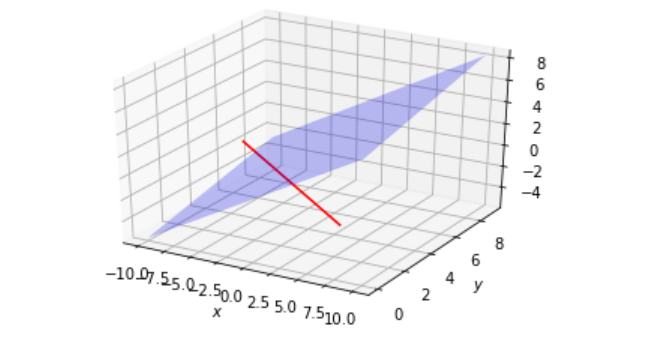
\includegraphics[width=\columnwidth]{figure.png}
    \caption{Hyperbola}
    \label{quadform/73/b/fig:hyperbola}
\end{figure}  
\end{enumerate}
\end{document}